% SOICT 2026 submission draft (v3) --- Springer LNCS format.
% v3 (2026-08-05): consolidation of three ablation studies. v2 established the classical HAR primary
% baseline (Table 1) and the news-branch ablation (Table 2). v3 adds two more ablations run overnight
% --- the cross-stock graph branch (docs/reports/2026-08-05_graph_ablation_results.md) and the
% per-ticker gate (docs/reports/2026-08-05_gate_ablation_results.md) --- and reframes the paper's
% contribution around what the three ablations jointly show: only the news features carry a
% paired-t-significant gain; the graph and gate mechanisms add no measurable value. v1 and v2 are
% frozen prior versions; do not edit them.
% Template: llncs.cls from https://soict.org/wp-content/uploads/2025/09/Latex-Template-for-Springer.zip
% NOTE: verify this llncs.cls/splncs04.bst pair against the official SOICT 2026 download before
% final submission. Bibliography entries marked [VERIFY] need bibliographic confirmation.
%
\documentclass[runningheads]{llncs}
%
\usepackage[T1]{fontenc}
\usepackage{graphicx}
\usepackage{amsmath}
\usepackage{booktabs}
\usepackage{tikz}
\usetikzlibrary{arrows.meta,positioning,fit,backgrounds}
%
% --- Canonical number macros (single source of truth; keeps sections consistent) ---
% Classical HAR baseline: linear regression on the three HAR scales, per-ticker 80/20 temporal
% split, pooled point-wise evaluation. Source: results/har_baseline_2026-08-05_224208/.
\newcommand{\qlikeHARc}{0.5493}
\newcommand{\rmseHARc}{0.002182}
\newcommand{\maeHARc}{0.000575}
\newcommand{\rsqHARc}{0.7419}
\newcommand{\diraccHARc}{48.65}
% Price-only LSTM--GAT backbone (no news branch): ablation control, 3-seed mean.
\newcommand{\qlikeBB}{0.4603}
\newcommand{\rmseBB}{0.002923}
\newcommand{\maeBB}{0.0008113}
\newcommand{\rsqBB}{0.7749}
\newcommand{\diraccBB}{48.47}
% Gated news fusion (full model): 3-seed mean.
\newcommand{\qlikeNews}{0.4430}
\newcommand{\rmseNews}{0.002734}
\newcommand{\maeNews}{0.0007930}
\newcommand{\rsqNews}{0.8031}
\newcommand{\diraccNews}{47.77}
% Ablation 1 (news branch) paired t-tests across 3 seeds (price-only backbone vs gated news fusion).
\newcommand{\qliketstat}{-6.22}
\newcommand{\rmsetstat}{-9.38}
\newcommand{\diracctstat}{-2.97}
% Ablation 2 (spatial/graph branch): identity adjacency (no cross-stock message passing) vs the
% real k-NN graph, on the price-only backbone, 3-seed mean. Source:
% docs/reports/2026-08-05_graph_ablation_results.md sec. 3.
\newcommand{\qlikeNoGraph}{0.4657}
\newcommand{\rmseNoGraph}{0.002788}
\newcommand{\maeNoGraph}{0.0007877}
\newcommand{\rsqNoGraph}{0.7953}
\newcommand{\diraccNoGraph}{48.29}
% Ablation 3 (gate mechanism): always-on news fusion (no gate) vs the per-ticker gate, 3-seed mean.
% The gated column equals the full news model above. Source:
% docs/reports/2026-08-05_gate_ablation_results.md.
\newcommand{\qlikeNoGate}{0.4366}
\newcommand{\rmseNoGate}{0.002723}
\newcommand{\maeNoGate}{0.0007873}
\newcommand{\rsqNoGate}{0.8047}
\newcommand{\diraccNoGate}{48.22}
% Paired-t critical value, two-sided 5%, df=2.
\newcommand{\tcrit}{4.30}
\newcommand{\nseed}{3}
\newcommand{\ntick}{33}
%
\begin{document}
%
\title{News Features Improve VN30 Volatility Magnitude Forecasts Independently of Graph and Gate Mechanisms}
%
\titlerunning{News-Feature Volatility Forecasting for VN30}
%
\author{Author One\inst{1} \and Author Two\inst{1}}
\authorrunning{Author One et al.}
%
\institute{VNUHCM University of Science, Ho Chi Minh City, Vietnam\\
\email{\{author1,author2\}@student.hcmus.edu.vn}}
%
\maketitle
%
\begin{abstract}
Volatility forecasts set risk limits and option prices for VN30, the most liquid stocks on
Vietnam's Ho Chi Minh Stock Exchange, yet price-only forecasters discard the Vietnamese-language news
that carries early information about volatility shocks. We augment a HAR-driven parallel LSTM--GAT
volatility backbone with a PhoBERT news branch and test which of its components improve the forecast.
Against the classical Heterogeneous Autoregressive (HAR) model, the standard econometric baseline for
daily volatility, the news model lowers five-day-ahead test QLIKE from \qlikeHARc{} to \qlikeNews{}
and raises $R^2$ from \rsqHARc{} to \rsqNews{}, while the classical HAR stays lower on absolute error
(RMSE \rmseHARc{} vs.\ \rmseNews{}). Three ablations, each over three seeds at a matched budget,
locate the source of the gain. Removing the news branch raises QLIKE and RMSE with a paired $t$-test
($t=\qliketstat$ and $t=\rmsetstat$, $|t|>\tcrit$). Removing the cross-stock graph (identity
adjacency) moves no metric past the 5\% threshold (all $|t|<1.9$). Removing the per-ticker gate
(always-on news fusion) also moves no metric past the threshold (all $|t|<2.3$), and the simpler
no-gate model is marginally better on every metric's mean. The news features carry the contribution;
the graph and gate mechanisms built around them add no measurable value, so a simpler architecture
matches the full one. Directional accuracy does not improve for any model (all near \diraccNews\%):
the day-to-day change in the single-day Parkinson estimator is anti-persistent (sign lag-1
autocorrelation $-0.30$, negative for all \ntick{} tickers), and model-free forecasters reach the
same $\approx 49\%$ ceiling at negative $R^2$. News improves the forecast magnitude a model can
learn, independently of graph-based sharing or per-ticker gating, and leaves untouched a direction
task that is near-random for every forecaster.

\keywords{Volatility forecasting \and Graph neural networks \and Financial news \and PhoBERT \and
Emerging markets.}
\end{abstract}
%
% ======================================================================
\section{Introduction}
% Stakes: who suffers and why the domain matters.
Volatility forecasts drive the daily risk decisions of every desk that trades VN30, the basket of
roughly thirty most liquid stocks on Vietnam's Ho Chi Minh Stock Exchange. A margin engine sizes
collateral from forecast volatility; an option desk prices from it; a risk officer sets position
limits against it. When the forecast tracks tomorrow's realized volatility poorly, each of these
decisions pays for the error. VN30 desks make these decisions in an information environment that a
price-only forecaster ignores: a steady flow of Vietnamese-language news, from official press and
from brokerage research, that plausibly signals volatility shocks before they show up in the price
range.

% Problem gap: structural limitation of current approaches.
Two limitations keep existing forecasters from using that signal. First, the workhorse econometric
model, the Heterogeneous Autoregressive (HAR) model of Corsi~\cite{corsi2009}, is linear and
univariate: it regresses future volatility on its own daily, weekly, and monthly averages, with no
channel for text and no channel for cross-stock coupling. Second, the deep-learning forecasters
that add cross-stock structure through graph neural networks~\cite{velickovic2018,sonani2025}
remain price-only, and the smaller line of text-augmented work fuses a single market-wide sentiment
score by concatenation, which admits the same amount of news to every stock. Whether a market like
VN30 needs richer machinery than uniform concatenation is an open question: a widely-covered bank
and a thinly-covered utility plausibly carry different news intensity, but no study has isolated
whether modeling that difference improves the forecast.

% Key abstraction.
We build a news-fusion forecaster and ask which of its added components improves the forecast. A
shared news branch encodes each stock's daily news into a vector. A \emph{per-ticker gate}, a single
learned scalar per stock passed through a sigmoid, scales that vector before it joins the price
representation, so the model can admit a different amount of news for each stock. A graph attention
network inside the price branch couples stocks through a $k$-nearest-neighbour graph. We then ablate
these three components one at a time, the news branch, the cross-stock graph, and the gate, to locate
where any forecast gain comes from.

% Design intuition.
The full model has two branches (Fig.~\ref{fig:arch}). A price branch reuses a fixed parallel
LSTM--GAT backbone: a per-stock long short-term memory (LSTM) network reads the three HAR
volatility scales over a 22-day window, and a graph attention network (GAT) mixes information
across stocks on a $k$-nearest-neighbour graph. A
news branch reads a 146-dimensional daily news vector per stock, built offline from PhoBERT
embeddings of Vietnamese articles, split into official-press and brokerage groups and carried
forward by an exponentially weighted average. The per-ticker gate scales the news branch, and a
final linear layer fuses the two branches into a five-day-ahead volatility forecast.

% Contributions.
This paper makes four contributions.
\begin{enumerate}
\item \textbf{Architecture.} We design a news-fusion volatility forecaster that gates a PhoBERT
dual-group news branch per stock and fuses it with a HAR-driven LSTM--GAT price backbone
(Section~\ref{sec:method}).
\item \textbf{News improves forecast magnitude over the classical HAR baseline.} The full model
lowers five-day-ahead QLIKE from \qlikeHARc{} to \qlikeNews{} and raises $R^2$ from \rsqHARc{} to
\rsqNews{} against the classical HAR econometric model, and an ablation that removes only the news
branch shows the branch lowers QLIKE and RMSE across three seeds with a paired $t$-test
($t=\qliketstat$ and $t=\rmsetstat$, Section~\ref{sec:results}). The classical HAR stays lower on
absolute error, which we report and explain.
\item \textbf{Only the news features earn their place.} Three ablations across three seeds isolate
the news branch, the cross-stock graph, and the per-ticker gate. Only the news branch changes the
metrics under a paired $t$-test; removing the cross-stock graph or the gate moves no metric past the
5\% threshold, and a simpler always-on-news model without the gate matches the full model on every
metric's mean (Section~\ref{sec:ablation}). The gain comes from the news features, not from the
graph or the gate built around them.
\item \textbf{Direction is near-random by construction.} No model improves directional accuracy, and
the $\approx 48\%$ figure is the intrinsic ceiling of the task: the daily Parkinson target's
day-to-day change is anti-persistent, and model-free forecasters reach the same ceiling
(Section~\ref{sec:results} and Section~\ref{sec:discussion}).
\end{enumerate}

% Results preview.
On \ntick{} VN30 tickers over a temporal split, the news model attains test $R^2=\rsqNews$,
above both the classical HAR baseline (\rsqHARc) and the price-only backbone (\rsqBB), and the QLIKE
and RMSE gains from news hold in the same direction on all three seeds of the ablation. Neither the
cross-stock graph nor the per-ticker gate adds a measurable increment on top of the news features:
each removed on its own leaves every metric within seed noise, which points toward a simpler
architecture. The directional-accuracy result reframes a metric that earlier drafts of this project
reported as high (68--72\%) but which a measurement artifact had inflated; the corrected figure is
near coin-flip, and we explain it as a property of the data (Section~\ref{sec:discussion}).

% ======================================================================
\section{Background and Problem Setup}
\label{sec:background}

\subsubsection{Parkinson volatility.}
We forecast daily volatility measured by the Parkinson range estimator, which uses the intraday
high $H$ and low $L$:
\begin{equation}
\sigma^2_{\text{Park}} = \frac{\left(\ln(H/L)\right)^2}{4\ln 2}.
\label{eq:parkinson}
\end{equation}
The range estimator uses more of the day's price path than a close-to-close estimator and is a
standard choice for daily data~\cite{parkinson1980}, and range-based inputs improve
realized-volatility forecasts within a HAR framework~\cite{korkusuz2023}. It is a noisy one-day
proxy for the latent volatility, a fact that Section~\ref{sec:discussion} shows matters for the
direction task.

\subsubsection{The HAR decomposition and baseline.}
The HAR model of Corsi~\cite{corsi2009} predicts future volatility from three moving averages of
past volatility, over a daily (1-day), weekly (5-day), and monthly (22-day) window. The three
scales approximate the long memory of volatility with a parsimonious linear regression, and the
model remains the benchmark that a new daily-volatility forecaster must beat. We use it two ways.
As features, the three averages are the input of the price branch, so the deep model starts from the
information HAR uses and adds temporal, cross-stock, and news structure on top. As a baseline, a
plain linear regression on the three averages is the classical HAR model we compare against in
Section~\ref{sec:results}.

\subsubsection{Forecast target and losses.}
For each stock and each day $t$ we predict the Parkinson volatility five trading days ahead, a
single-day value at $t+5$ (not a five-day average). We train with mean squared error on
normalized targets and evaluate on the original scale with the six metrics the project mandates:
MSE, RMSE, MAE, $R^2$, QLIKE, and directional accuracy. QLIKE, the quasi-likelihood loss standard
in the realized-volatility literature~\cite{patton2011}, penalizes under-prediction of volatility
more than over-prediction and tolerates the noise in the volatility proxy:
\begin{equation}
\text{QLIKE} = \frac{1}{T}\sum_{t=1}^{T}\left(\frac{\hat{\sigma}^2_t}{\sigma^2_t}
 - \ln\frac{\hat{\sigma}^2_t}{\sigma^2_t} - 1\right).
\label{eq:qlike}
\end{equation}
Directional accuracy measures how often the predicted change in volatility from one step to the
next matches the realized change in sign. We compute it \emph{per ticker over time}: for each
stock we compare $\operatorname{sign}(\hat{y}_{i,t+1}-\hat{y}_{i,t})$ against
$\operatorname{sign}(y_{i,t+1}-y_{i,t})$, then average across stocks. Section~\ref{sec:results}
explains why the naive alternative, which flattens all stocks and days into one array before taking
differences, reports a misleadingly high number.

% ======================================================================
\section{Method: Per-Ticker Gated News Fusion}
\label{sec:method}

The model reads two aligned inputs per 22-day window: a price tensor of HAR features and a news
tensor of PhoBERT-derived features, both indexed by stock and day. Two branches encode them
independently, a per-ticker gate scales the news branch, and a linear layer fuses the result into
one forecast per stock. Figure~\ref{fig:arch} shows the flow; we describe the price branch, the
news branch, the gate, and the fusion in turn. Section~\ref{sec:ablation} ablates each of these
components in isolation.

\begin{figure}[t]
\centering
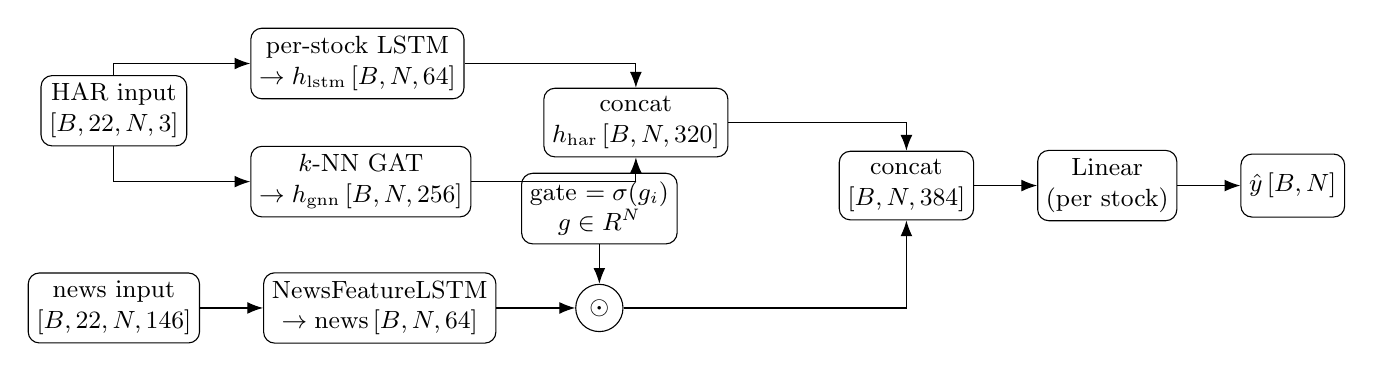
\begin{tikzpicture}[
  font=\small,
  box/.style={draw, rounded corners, align=center, minimum height=8mm, inner sep=3pt},
  op/.style={draw, circle, inner sep=1pt, minimum size=6mm},
  >={Latex[length=2mm]}
]
% price branch
\node[box] (harin) {HAR input\\ $[B,22,N,3]$};
\node[box, right=8mm of harin, yshift=6mm] (lstm) {per-stock LSTM\\ $\to h_{\text{lstm}}\,[B,N,64]$};
\node[box, right=8mm of harin, yshift=-9mm] (gat) {$k$-NN GAT\\ $\to h_{\text{gnn}}\,[B,N,256]$};
\node[box, right=10mm of lstm, yshift=-7.5mm] (harembed) {concat\\ $h_{\text{har}}\,[B,N,320]$};
% news branch
\node[box, below=16mm of harin] (newsin) {news input\\ $[B,22,N,146]$};
\node[box, right=8mm of newsin] (newslstm) {NewsFeatureLSTM\\ $\to \text{news}\,[B,N,64]$};
\node[op, right=10mm of newslstm] (mult) {$\odot$};
\node[box, above=5mm of mult] (gate) {gate $=\sigma(g_i)$\\ $g\in\mathbb{R}^{N}$};
% fusion
\node[box, right=14mm of harembed, yshift=-8mm] (concat) {concat\\ $[B,N,384]$};
\node[box, right=8mm of concat] (fuse) {Linear\\ (per stock)};
\node[box, right=8mm of fuse] (pred) {$\hat{y}\,[B,N]$};
% edges price
\draw[->] (harin) |- (lstm);
\draw[->] (harin) |- (gat);
\draw[->] (lstm) -| (harembed);
\draw[->] (gat) -| (harembed);
\draw[->] (harembed) -| (concat);
% edges news
\draw[->] (newsin) -- (newslstm);
\draw[->] (newslstm) -- (mult);
\draw[->] (gate) -- (mult);
\draw[->] (mult) -| (concat);
% fusion
\draw[->] (concat) -- (fuse);
\draw[->] (fuse) -- (pred);
\end{tikzpicture}
\caption{The per-ticker gated news-fusion model. The price branch (top) reuses a fixed parallel
LSTM--GAT backbone; the news branch (bottom) encodes PhoBERT features, which a learned gate
$\sigma(g_i)$ scales per stock before concatenation. $B$ is batch size, $N$ the number of stocks.}
\label{fig:arch}
\end{figure}

\subsection{Price branch: a fixed HAR LSTM--GAT backbone}
The price branch reuses, read-only, the parallel LSTM--GAT backbone of the project, adapted from the
hybrid LSTM--GNN design of Sonani et al.~\cite{sonani2025}. Its input is a tensor
$[B,22,N,3]$: a batch of $B$ windows, each covering 22 trading days for $N$ stocks with the three
HAR volatility scales. A per-stock LSTM (input size 3, hidden size 64, two layers, dropout 0.2)
encodes each stock's temporal path into $h_{\text{lstm}}\in\mathbb{R}^{B\times N\times 64}$. In
parallel, a two-layer graph attention network (four heads, hidden size 64) mixes information across
stocks on a $k$-nearest-neighbour graph built from return correlation, and a mean over the time
axis yields $h_{\text{gnn}}\in\mathbb{R}^{B\times N\times 256}$. Concatenating the two gives the
price representation $h_{\text{har}}\in\mathbb{R}^{B\times N\times 320}$. Used alone, with a dense
head and no news branch, this backbone is the price-only backbone we ablate against in
Section~\ref{sec:results}; every news model reuses its embeddings without changing a weight, so the
ablation isolates the news contribution.

\subsection{News branch: dual-group PhoBERT features}
\label{sec:news}
The news branch consumes a 146-dimensional vector per stock per day, computed offline so that
training reads a cache rather than a language model. We build the vector in four steps.

\emph{Encode.} Each Vietnamese article (title and lead) passes once through
PhoBERT~\cite{phobert2020}, a BERT model~\cite{devlin2019} pre-trained on Vietnamese, yielding a
768-dimensional embedding cached by URL.

\emph{Attribute and reduce.} An article that names several stocks copies its embedding to each named
stock. Principal component analysis (PCA), fit only on data before the training cutoff to avoid
leakage, reduces each embedding to 32 dimensions.

\emph{Aggregate per stock-day.} When a stock has several articles on one day, we average their
32-dimensional vectors dimension by dimension into a single vector, and sum per-topic article counts
over seven topic categories (earnings, dividend, M\&A, management, regulation, macro, sector).

\emph{Split and carry forward.} We keep two source groups separately: an official-press group
(general news outlets) and a brokerage group (securities-firm research), so the model can weigh the
two differently. Because most days carry no fresh article for a given stock, we add an
exponentially weighted average of each group with a 30-trading-day half-life. On a day with no new
article the average decays by a factor $1-\alpha$ with $\alpha=1-\exp(-\ln 2/30)\approx 0.0228$;
on a day with an article it updates toward the new value. The half-life encodes the persistence of
a news effect: a report keeps some relevance for weeks rather than vanishing the next day. The 146
features are 32 embedding dimensions plus a norm for each of the two groups (66), the same for the
two exponentially weighted averages (66), and 14 topic counts.

A one-layer encoder maps this vector to a news representation. A linear layer
($146\to 64$) with a ReLU feeds a single-layer LSTM ($64\to 64$) over the 22-day window, producing
$\text{news}\in\mathbb{R}^{B\times N\times 64}$. The encoder processes each stock independently.

\subsection{The per-ticker gate}
\label{sec:gate}
A single scalar per stock controls how much news that stock admits. We hold a parameter vector
$g\in\mathbb{R}^{N}$, pass it through a sigmoid to get a gate in $(0,1)$ per stock, and scale the
news representation elementwise:
\begin{equation}
\text{news}^{\text{gated}}_{i} = \sigma(g_i)\cdot \text{news}_{i}, \qquad i=1,\dots,N.
\label{eq:gate}
\end{equation}
The gate does not depend on the day's input; it is one learned number per stock. Because the news
encoder processes stocks independently, the gate scales elementwise, and the fusion layer applies
per stock, the gradient of $g_i$ depends only on stock $i$'s own data. A unit test confirms this
isolation: changing another stock's label leaves $\partial\mathcal{L}/\partial g_i$ unchanged. We
give the gate its own optimizer group with a learning rate of 0.05, ten times the rate of the rest
of the network, so the gates move enough within the 20-epoch budget.

\subsection{Fusion}
Concatenating the price representation with the gated news representation gives
$[B,N,384]$, and a linear layer applied per stock produces the forecast
$\hat{y}\in\mathbb{R}^{B\times N}$, one five-day-ahead volatility value per stock per window. The
graph attention layer is the only place stocks exchange information, and it sits inside the price
branch, before the gate. From the gate onward the model treats stocks independently.

% ======================================================================
\section{Experimental Setup}
\label{sec:setup}

\subsubsection{Universe and split.}
We use \ntick{} VN30 constituents with daily open-high-low-close-volume (OHLCV) data. Series lengths range from about 1{,}300
sessions (SSB, listed 2021) to about 4{,}900 (VNM, ACB, from 2006). We exclude two current VN30
members, BSR and VPL, because their listing histories are too short to align with the panel: VPL
had 99 trading sessions and BSR 401 at data cutoff, and the graph model requires every stock to
have data on each shared date, so including VPL would shrink the common window to about 58 trading
days. For the deep models we split each series chronologically into 70\% train, 15\% validation, and
15\% test to prevent look-ahead leakage, and we fit all normalizers and the news PCA on the training
portion only.

\subsubsection{Baselines and what each comparison controls.}
We compare the full model against two references. The classical HAR baseline is an ordinary linear
regression of the five-day-ahead target on the three HAR volatility scales, fit per ticker on the
chronologically-early 80\% of that ticker's rows and evaluated point-wise on the late 20\%; it is
the field-standard econometric benchmark and answers whether the deep news architecture beats the
model practitioners already use. The price-only backbone is the same LSTM--GAT model as the full
system with the news branch removed; it shares the deep model's data, split, seeds, epoch budget,
and batch configuration, and differs only in the news branch and its gate. The backbone comparison
is therefore a controlled ablation: a gain attributes to news fusion, not to a training-setup
difference. The classical HAR uses a point-wise 80/20 split rather than the windowed 70/15/15 split
of the deep models, so we read it as a reference benchmark and rest the causal claim about the news
branch on the ablation.

\subsubsection{Training and ablation protocol.}
We train the deep models for 20 epochs with the Adam optimizer~\cite{kingma2015}, a two-group
learning rate (0.005 main, 0.05 gate), dropout 0.2, and early stopping on validation loss. We
normalize HAR features and targets with statistics from the training split and invert the transform
before computing metrics on the original volatility scale. To move from a single run to a comparison
we can defend, we repeat every ablation condition on three independent seeds (42, 123, 2026) at this
identical budget and report the mean, standard deviation, and a paired $t$-test across seeds. Each
ablation removes one component and holds the data, split, seeds, budget, and remaining architecture
fixed, so a change in a metric attributes to that component alone. We report results from the
pipeline after two corrections described in Section~\ref{sec:results}; earlier deep baselines in
the project predate those corrections and are not directly comparable, so we exclude them from the
comparison.

% ======================================================================
\section{Results}
\label{sec:results}

\subsection{News fusion improves QLIKE and \texorpdfstring{$R^2$}{R2} over the classical HAR baseline}
Table~\ref{tab:headline} reports the five-day-ahead test metrics for the classical HAR baseline and
the gated news model. The news model lowers QLIKE from \qlikeHARc{} to \qlikeNews{} and raises $R^2$
from \rsqHARc{} to \rsqNews{}, so it fits the volatility level better and matches the QLIKE loss
that risk and option desks care about more closely. The classical HAR is not dominated: it attains
lower RMSE (\rmseHARc{} vs.\ \rmseNews{}) and lower MAE (\maeHARc{} vs.\ \maeNews{}). The linear
model, fit directly to minimize squared error on the raw scale, is hard to beat on plain squared and
absolute error, while the deep model wins on the proportional QLIKE loss and on explained variance.
Directional accuracy is near coin-flip for both (\diraccHARc\% vs.\ \diraccNews\%), a point
Section~\ref{sec:refbaselines} shows holds for every forecaster.

\begin{table}[t]
\caption{Five-day-ahead test metrics: classical HAR baseline vs.\ the full gated news-fusion model.
The news model is the mean over three seeds (42, 123, 2026); the classical HAR is a single
deterministic fit. Lower is better for QLIKE, RMSE, MAE; higher for $R^2$ and directional accuracy
(DirAcc). Bold marks the better value per row. The classical HAR uses a point-wise 80/20 per-ticker
split; the deep model uses a windowed 70/15/15 split, so this is a reference comparison and the
controlled news effect is the ablation in Table~\ref{tab:ablation}.}
\label{tab:headline}
\centering
\begin{tabular}{lcc}
\toprule
Metric & Classical HAR & Gated news fusion \\
\midrule
QLIKE            & $0.5493$              & $\mathbf{0.4430\pm0.0185}$ \\
RMSE             & $\mathbf{0.002182}$   & $0.002734\pm0.000096$ \\
MAE              & $\mathbf{0.000575}$   & $0.0007930$ \\
$R^2$            & $0.7419$              & $\mathbf{0.8031\pm0.0139}$ \\
DirAcc (\%)      & $\mathbf{48.65}$      & $47.77\pm0.52$ \\
\bottomrule
\end{tabular}
\end{table}

\smallskip
\noindent\textbf{Takeaway.} The deep news model improves the loss that the volatility literature
treats as primary (QLIKE) and the variance explained ($R^2$) over the classical HAR benchmark, but
does not uniformly dominate it: the linear baseline keeps lower RMSE and MAE. We report the mixed
result plainly and turn to a three-part ablation to measure what each component of the deep model
buys.

\subsection{Ablation study: only the news branch changes the metrics}
\label{sec:ablation}
The deep model adds three components to a plain per-stock LSTM: a news branch, a cross-stock graph
in the price branch, and a per-ticker gate on the news branch. Three ablations, each over the same
three seeds and 20-epoch budget, remove one component at a time. Only the news branch moves the
metrics under a paired $t$-test.

\subsubsection{Ablation 1: the news branch lowers QLIKE and RMSE.}
We compare the full model against the price-only backbone that shares every other component, over
the same three seeds. Table~\ref{tab:ablation} reports the result. Removing the news branch raises
QLIKE from \qlikeNews{} to \qlikeBB{} and RMSE from \rmseNews{} to \rmseBB{}; equivalently, adding it
lowers both. A paired $t$-test across the three seeds gives $t=\qliketstat$ for QLIKE and
$t=\rmsetstat$ for RMSE, both past the two-sided 5\% threshold for two degrees of freedom
($|t|>\tcrit$). The gains hold in the same direction on every seed: per-seed QLIKE differences are
$-0.0198$, $-0.0204$, and $-0.0118$, and per-seed RMSE differences are $-0.000183$, $-0.000228$, and
$-0.000159$. The news branch also raises $R^2$ from \rsqBB{} to \rsqNews{} and lowers MAE from
\maeBB{} to \maeNews{}.

\begin{table}[t]
\caption{Ablation 1, news branch: five-day-ahead test metrics, mean$\pm$std over three seeds
(42, 123, 2026), 20 epochs each. The two rows share the LSTM--GAT backbone, data, split, seeds, and
budget; they differ only in the news branch and gate. Lower is better for QLIKE, RMSE, MAE; higher
for $R^2$ and DirAcc. The paired $t$ is across the three seeds; $|t|>\tcrit$ passes at the 5\% level
with two degrees of freedom.}
\label{tab:ablation}
\centering
\begin{tabular}{lccc}
\toprule
Metric & Price-only backbone & Gated news fusion & Paired $t$ (n=3) \\
\midrule
QLIKE            & $0.4603\pm0.0205$   & $\mathbf{0.4430\pm0.0185}$   & $-6.22$ (sig.) \\
RMSE             & $0.002923\pm0.000090$ & $\mathbf{0.002734\pm0.000096}$ & $-9.38$ (sig.) \\
MAE              & $0.0008113$         & $\mathbf{0.0007930}$         & n/a \\
$R^2$            & $0.7749\pm0.0140$   & $\mathbf{0.8031\pm0.0139}$   & n/a \\
DirAcc (\%)      & $\mathbf{48.47\pm0.35}$ & $47.77\pm0.52$           & $-2.97$ (n.s.) \\
\bottomrule
\end{tabular}
\end{table}

\subsubsection{Ablation 2: the cross-stock graph changes nothing.}
The price branch mixes stocks through a graph attention network on a $k$-nearest-neighbour graph
built from return correlation. To test whether that cross-stock structure does measurable work, we
replace the real adjacency with an identity matrix, so each node attends only to itself; the
architecture and parameter count stay fixed, and only message passing across stocks disappears. A
sanity check confirms the substitution: under the identity adjacency, perturbing every other stock's
input leaves a target stock's graph embedding unchanged (maximum change $0.0$), while under the real
graph the same perturbation changes it (maximum change $2.32$). Table~\ref{tab:graphablation} reports
the result on the price-only backbone. No metric passes the 5\% threshold: every paired $t$ across
the three seeds has $|t|<\tcrit$, and the differences are small and inconsistent in sign. The real
graph is marginally lower on QLIKE and higher on DirAcc, while the identity variant is marginally
lower on RMSE and MAE and higher on $R^2$; all gaps sit within the seed-to-seed standard deviation.
The graph's cross-stock message passing, as encoded by this static $k$-NN adjacency, is not a
measurable driver of forecast quality; the spatial branch's contribution comes from its per-node
capacity, not from coupling stocks.

\begin{table}[t]
\caption{Ablation 2, cross-stock graph: five-day-ahead test metrics on the price-only backbone,
mean$\pm$std over three seeds, 20 epochs each. The identity-adjacency column removes all cross-stock
message passing at the same parameter count; the $k$-NN column is the real return-correlation graph.
The paired $t$ is across the three seeds (identity $-$ $k$-NN); every $|t|<\tcrit$ fails the 5\%
threshold at two degrees of freedom, so we mark no value.}
\label{tab:graphablation}
\centering
\begin{tabular}{lccc}
\toprule
Metric & Identity (no graph) & $k$-NN graph & Paired $t$ (n=3) \\
\midrule
QLIKE            & $0.4657\pm0.0112$     & $0.4603\pm0.0205$     & $+0.30$ (n.s.) \\
RMSE             & $0.002788\pm0.000058$ & $0.002923\pm0.000090$ & $-1.64$ (n.s.) \\
MAE              & $0.0007877$           & $0.0008113$           & $-1.89$ (n.s.) \\
$R^2$            & $0.7953\pm0.0085$     & $0.7749\pm0.0140$     & $+1.63$ (n.s.) \\
DirAcc (\%)      & $48.29\pm0.04$        & $48.47\pm0.35$        & $-0.98$ (n.s.) \\
\bottomrule
\end{tabular}
\end{table}

\subsubsection{Ablation 3: the per-ticker gate changes nothing.}
The per-ticker gate scales each stock's news branch by a learned scalar. To test whether this
adaptive admission helps, we compare the gated model against an always-on variant that concatenates
the same news branch with no gate, so every stock admits its news fully. The two architectures are
identical apart from the gate. Table~\ref{tab:gateablation} reports the result. No metric passes the
5\% threshold (all $|t|<\tcrit$), and the simpler no-gate model is marginally lower on QLIKE, RMSE,
and MAE and marginally higher on $R^2$ and DirAcc, better on every mean. The sign of the gate's
effect on the continuous-error metrics flips across seeds: the gate helps on seed 123 and hurts on
seeds 42 and 2026. The per-ticker gate does not recover accuracy beyond what always-on news fusion
already attains.

\begin{table}[t]
\caption{Ablation 3, per-ticker gate: five-day-ahead test metrics, mean$\pm$std over three seeds,
20 epochs each. The no-gate column is the always-on news-fusion variant (same news branch, no gate);
the gated column is the full model. The paired $t$ is across the three seeds (gated $-$ no-gate);
every $|t|<\tcrit$ fails the 5\% threshold at two degrees of freedom. The no-gate variant is
marginally better on every mean, so we mark no value.}
\label{tab:gateablation}
\centering
\begin{tabular}{lccc}
\toprule
Metric & No gate (always-on) & Per-ticker gate & Paired $t$ (n=3) \\
\midrule
QLIKE            & $0.4366\pm0.0116$     & $0.4430\pm0.0185$     & $+1.24$ (n.s.) \\
RMSE             & $0.002723\pm0.000074$ & $0.002734\pm0.000096$ & $+0.37$ (n.s.) \\
MAE              & $0.0007873$           & $0.0007930$           & $+1.01$ (n.s.) \\
$R^2$            & $0.8047\pm0.0106$     & $0.8031\pm0.0139$     & $-0.39$ (n.s.) \\
DirAcc (\%)      & $48.22\pm0.27$        & $47.77\pm0.52$        & $-2.28$ (n.s.) \\
\bottomrule
\end{tabular}
\end{table}

\smallskip
\noindent\textbf{Takeaway.} Of the three components, only the news branch changes the metrics that
survive a paired test. The cross-stock graph and the per-ticker gate, each removed on its own, cost
nothing measurable: a plain per-stock LSTM with always-on news concatenation matches the full
architecture within seed noise on every metric. The finding argues for architectural parsimony,
because the news features carry the gain and the two mechanisms designed to use them more cleverly do
not add to it. Three seeds is the minimum for a paired $t$-test, so we do not read the two null
results as proof of equivalence; the differences are small and consistent in sign across all three
ablations, which supports the parsimony reading qualitatively. We ablate one component at a time and
do not test removing the graph and the gate jointly.

\subsection{News does not improve direction}
Directional accuracy tells the opposite story. In the news-branch ablation both models sit near
48\%, below the 50\% no-skill line; the per-seed differences ($-0.53$, $-1.18$, $-0.42$ percentage
points, favouring the backbone) give a paired $t$ of $\diracctstat$, short of the 5\% threshold.
News neither helps nor reliably hurts direction, and the graph and gate ablations move it no further.

\subsection{A measurement correction behind these numbers}
Two corrections separate the deep-model numbers from earlier project reports. First, an earlier
directional accuracy of 68--72\% came from flattening predictions and targets into one $[\text{window},
\text{stock}]$ array before differencing, so most comparisons ran across different stocks on the
same day rather than the same stock across time; same-day cross-stock comparisons benefit from
market-wide co-movement and inflate the score. The per-ticker metric of
Section~\ref{sec:background} removes this artifact and drops the figure to the intrinsic level.
Second, the backbone's feature normalizer had been fit but never applied, so earlier models trained
on raw, unnormalized volatility; applying it moved the headline QLIKE from about 0.55 to about 0.46.
We report only post-correction numbers.

\subsection{Direction is near-random for every forecaster}
\label{sec:refbaselines}
To show the low directional accuracy is a property of the target rather than of any one model, we
run two model-free reference forecasters against the identical per-ticker metric and target
construction, alongside the three trained models. Table~\ref{tab:refs} gives the result. Persistence
(predict the last observed volatility) reaches 49.5\% direction, and a five-day trailing mean
reaches 49.1\%, both statistically indistinguishable from the trained models near 48\%. No
forecaster, naive or trained, beats coin-flip on this direction task. Yet the classical HAR and both
deep models attain positive $R^2$ (0.74 to 0.79) while both naive forecasters have \emph{negative}
$R^2$, so every fitted model does real work on the volatility level while every forecaster fails on
the day-to-day sign.

\begin{table}[t]
\caption{Directional accuracy and $R^2$ against the identical five-day target, per ticker, averaged
over \ntick{} tickers. The two reference forecasters use no learned parameters. The three trained
rows are single reference runs (seed 42 for the deep models) used for this like-for-like comparison;
the deep models' three-seed means (Table~\ref{tab:ablation}) are 48.5\% and 47.8\% for direction and
\rsqBB{}/\rsqNews{} for $R^2$, consistent within seed noise. Direction is near 49\% for all five;
only the fitted models attain positive $R^2$.}
\label{tab:refs}
\centering
\begin{tabular}{lcc}
\toprule
Forecaster & Mean per-ticker DirAcc (\%) & Mean $R^2$ \\
\midrule
Persistence (last observed) & 49.5 & $-0.64$ \\
Trailing mean (5-day)       & 49.1 & $-0.08$ \\
Classical HAR (linear)      & 48.7 & $+0.742$ \\
Price-only backbone (trained) & 48.1 & $+0.759$ \\
Gated news fusion (trained) & 47.6 & $+0.787$ \\
\bottomrule
\end{tabular}
\end{table}

\smallskip
\noindent\textbf{Takeaway.} Every fitted model forecasts the volatility level well and the
day-to-day direction no better than chance, because the direction of the daily target is close to
unpredictable for anyone. Section~\ref{sec:discussion} explains why.

% ======================================================================
\section{Discussion}
\label{sec:discussion}

\subsection{Why direction is near-random}
The forecast target is the single-day Parkinson estimator, and its day-to-day change is
anti-persistent. Measured on the full series of each stock, the sign of the daily change in
Parkinson volatility has a lag-1 autocorrelation of $-0.30$ on average, negative for all \ntick{}
tickers (range $-0.34$ to $-0.24$). An up-move in daily volatility tends to precede a
down-move: the estimator oscillates day to day around a slowly drifting level, a known property of
range-based daily volatility proxies. A forecaster that produces a smooth estimate of the level
cannot reproduce this high-frequency oscillation, so its directional calls decouple from the target
and sit at or just below 50\%. The per-ticker spread is tight (standard deviation about one
percentage point, 27 of \ntick{} tickers inside 48--52\%), so the near-random result is a shared
property of the universe rather than a few pathological stocks. News cannot rescue this direction
task because the task is near-random for structural reasons, and we base our conclusions on the
continuous-error metrics that reflect what the model can forecast.

\subsection{Why the classical HAR keeps lower RMSE}
The classical HAR baseline attains lower RMSE and MAE than the deep model even though the deep model
wins on QLIKE and $R^2$. Two forces explain the split. The linear regression minimizes squared
error on the raw target scale directly, so it optimizes the quantity RMSE measures, while
the deep model trains on normalized targets and optimizes a representation that also serves the
proportional QLIKE loss the volatility literature favours. The two baselines also use different
evaluation protocols (point-wise 80/20 for HAR, windowed 70/15/15 for the deep model), which shifts
the test window and the pooling. We therefore read the HAR comparison as a benchmark against the
standard econometric model and rely on the ablation, which holds the protocol fixed, for the causal
statement that news lowers QLIKE and RMSE.

\subsection{Parsimony: the news features, not the mechanisms around them}
The three ablations converge on one reading. The news branch carries a QLIKE and RMSE gain that
survives a paired $t$-test across seeds; the cross-stock graph and the per-ticker gate, each removed
on its own, leave every metric within seed noise. A simpler architecture, a per-stock LSTM with
always-on news concatenation, matches the full model on every metric's mean. The gate fails a second
test as well: its learned per-stock values do not line up with independent measures of which stocks
should need news. Four methods (two feature-importance analyses, an ablation on per-stock QLIKE
change, and the learned gate itself) rank the stocks differently, so the gate does not double as a
readout of per-stock news relevance. Neither on aggregate accuracy nor on interpretability does the
gate earn its added parameters here. We read this as a case for admitting news simply and spending
model complexity elsewhere, while noting the sample-size caveat: three seeds is the minimum for a
paired $t$-test, so the two null ablations bound the effect rather than prove its absence.

\subsection{A preliminary observation on forecast horizon}
An exploratory sweep over 1, 10, and 22-day horizons suggested that the news advantage concentrates
at short horizons and fades or reverses by 22 days, which a decay analysis would explain: the
30-day half-life news feature is nearly constant across these horizons, while volatility's own
predictability mean-reverts within days, so the room for a news increment shrinks as the horizon
grows. We flag this as preliminary only. The 1, 10, and 22-day runs predate the two corrections of
Section~\ref{sec:results} and have not been re-run on the corrected pipeline, so we do not state the
horizon reversal as a settled result. The structural evidence (news feature autocorrelation of 0.72
at 22 days versus volatility autocorrelation of 0.12) comes from raw data outside the training
pipeline, which the corrections do not touch, but the model comparison itself needs a
corrected, multi-seed re-run before we can cite it.

% ======================================================================
\section{Related Work}
\label{sec:related}

We place related work after the evaluation because the contribution is empirical: what news buys, and
what the graph and gate do not, is visible only once the head-to-head numbers are on the table. Prior
work falls into three groups.

\subsubsection{Econometric volatility models.}
The HAR model~\cite{corsi2009} and its range-based inputs~\cite{parkinson1980} set the standard for
daily volatility forecasting and remain hard to beat; in our own evaluation the classical HAR keeps
lower RMSE and MAE than the deep model. They are linear and univariate: no channel admits text, and
no channel couples one stock to another. We keep their multi-scale features as the input of the
price branch and add the news channel they omit, gaining on QLIKE and $R^2$.

\subsubsection{Deep and graph-based forecasters.}
LSTM forecasters~\cite{hochreiter1997} capture nonlinear temporal structure, and graph attention
networks~\cite{velickovic2018} model cross-asset coupling; hybrid LSTM--GNN designs combine both for
stock prediction~\cite{sonani2025}. These forecasters remain price-only. Our price branch adopts the
hybrid LSTM--GNN backbone, though our ablation finds that the cross-stock graph adds no measurable
value on this VN30 panel: the graph's benefit over a per-node transform sits within seed noise. We
therefore adopt the backbone for its per-node capacity and locate the paper's contribution in the
news channel these designs lack, not in the graph structure.

\subsubsection{News- and text-augmented forecasting.}
Text-augmented forecasters add sentiment scores or news embeddings: an Attention-LSTM with a news
opinion index warns of systemic risk in China~\cite{ouyang2021}, and a growing line couples
sentiment analysis with graph neural networks for stock prediction~\cite{das2024}. These designs
usually fuse a single market-wide signal by concatenation, on English- or Chinese-language markets.
We work in Vietnamese with PhoBERT~\cite{phobert2020} on VN30, an emerging market where
news-augmented volatility forecasting is little-studied, and we test whether a per-ticker gate that
admits a different amount of news per stock improves on uniform concatenation. On this panel it does
not: always-on concatenation matches the gate within seed noise. The contribution is an empirical
finding for a Vietnamese market: news features help continuous-error accuracy, the per-asset gating
mechanism does not.

% ======================================================================
\section{Limitations and Conclusion}
\label{sec:conclusion}

\subsubsection{Limitations.}
Four limitations bound the claims. First, three seeds is the minimum for a paired $t$-test; five or
more would strengthen both the positive news-branch result and the two null ablations, which bound
the graph and gate effects rather than prove them absent. Second, the classical HAR baseline uses a
point-wise 80/20 split while the deep models use a windowed 70/15/15 split, so the headline HAR
comparison is a reference benchmark rather than a protocol-matched control; the causal news claim
rests on the ablation, which holds the protocol fixed. Third, the \ntick{}-ticker universe differs slightly
from the official VN30 constituents (it keeps five long-history names that left the index and
excludes two short-history current members), so the dataset is a fixed, point-in-time VN30-like
universe rather than the live index. Fourth, we ablate the graph and the gate one at a time and do
not test removing them jointly, and the horizon observation of Section~\ref{sec:discussion} is
preliminary and needs a corrected re-run.

\subsubsection{Conclusion.}
Vietnamese news lowers five-day-ahead QLIKE and raises $R^2$ for a HAR-driven volatility forecaster
on VN30, against the classical HAR econometric baseline, though the linear HAR stays lower on
absolute error. Three ablations locate the gain: the news branch carries it with a paired $t$-test
across seeds, while the cross-stock graph and the per-ticker gate add no measurable value, so a
simpler architecture matches the full one. No model improves directional accuracy, and no forecaster
does: the day-to-day direction of daily Parkinson volatility is anti-persistent and near-random for
structural reasons. News improves the volatility magnitude a model can learn, independently of
graph-based sharing or per-ticker gating, and leaves untouched a direction task that the data itself
makes unlearnable. For a Vietnamese emerging market, this maps out both what news buys and which
mechanisms around it do not pay their way.

% NOTE FOR RIVF 2026 (secondary target, IEEE two-column, ~6 pages, EDAS): this LNCS draft needs a
% roughly 40--50% compression pass and a reformat to the IEEE class before that submission. Do not
% maintain two parallel documents; compress from this one when the RIVF timeline is confirmed.

%
% ---- Bibliography ----
% BibTeX users: \bibliographystyle{splncs04}. Entries below are hand-written for the draft; verify
% every [VERIFY] entry's exact venue/volume/pages/DOI before submission.
%
\begin{thebibliography}{99}

\bibitem{corsi2009}
Corsi, F.: A simple approximate long-memory model of realized volatility.
Journal of Financial Econometrics \textbf{7}(2), 174--196 (2009).
% [VERIFY] DOI 10.1093/jjfinec/nbp001 --- confirm volume/issue/pages.

\bibitem{parkinson1980}
Parkinson, M.: The extreme value method for estimating the variance of the rate of return.
The Journal of Business \textbf{53}(1), 61--65 (1980).
% [VERIFY] confirm volume/issue/pages.

\bibitem{patton2011}
Patton, A.J.: Volatility forecast comparison using imperfect volatility proxies.
Journal of Econometrics \textbf{160}(1), 246--256 (2011).
% [VERIFY] confirm as the QLIKE robust-loss reference; volume/pages.

\bibitem{hochreiter1997}
Hochreiter, S., Schmidhuber, J.: Long short-term memory.
Neural Computation \textbf{9}(8), 1735--1780 (1997).

\bibitem{velickovic2018}
Veli\v{c}kovi\'c, P., Cucurull, G., Casanova, A., Romero, A., Li\`o, P., Bengio, Y.:
Graph attention networks. In: International Conference on Learning Representations (ICLR) (2018).

\bibitem{devlin2019}
Devlin, J., Chang, M.-W., Lee, K., Toutanova, K.: BERT: Pre-training of deep bidirectional
transformers for language understanding. In: NAACL-HLT, pp. 4171--4186 (2019).

\bibitem{phobert2020}
Nguyen, D.Q., Nguyen, A.T.: PhoBERT: Pre-trained language models for Vietnamese.
In: Findings of the Association for Computational Linguistics: EMNLP 2020, pp. 1037--1042 (2020).
% [VERIFY] confirm page range.

\bibitem{kingma2015}
Kingma, D.P., Ba, J.: Adam: A method for stochastic optimization.
In: International Conference on Learning Representations (ICLR) (2015).

\bibitem{sonani2025}
Sonani, M.S., Badii, A., Moin, A.: Stock price prediction using a hybrid LSTM--GNN model:
integrating time-series and graph-based analysis. arXiv preprint arXiv:2502.15813 (2025).
% Verified against the source PDF (docs/paper/2502.15813v1.pdf): title, authors, arXiv id.

\bibitem{korkusuz2023}
Korkusuz, B., Kambouroudis, D., McMillan, D.G.: Do extreme range estimators improve realized
volatility forecasts? Evidence from G7 stock markets.
Finance Research Letters \textbf{55}, 103992 (2023).
% Verified against the source PDF (docs/paper/1-s2.0-S1544612323003641-main.pdf).

\bibitem{ouyang2021}
Ouyang, Z.-S., Yang, X.-T., Lai, Y.: Systemic financial risk early warning of financial market in
China using an Attention-LSTM model.
The North American Journal of Economics and Finance \textbf{56}, 101383 (2021).
% Verified against the source PDF (docs/paper/1-s2.0-S106294082100019X-main.pdf).

\bibitem{das2024}
Das, N., Sadhukhan, B., Chatterjee, R., Chakrabarti, S.: Integrating sentiment analysis with graph
neural networks for enhanced stock prediction: a comprehensive survey.
Decision Analytics Journal \textbf{10}, 100417 (2024).
% Verified against the source PDF (docs/paper/1-s2.0-S2772662224000213-main.pdf).

\end{thebibliography}
\end{document}
